\documentclass{article}
\usepackage{graphicx} 
\usepackage{geometry}
\usepackage{longtable}
\usepackage{caption}  
\usepackage{svg} 

\title{Design of the Electromagnetic Spectrum Monitoring System}
\author{Yeison N. Cardona A.}
\date{August 2024}

\begin{document}

\maketitle

\section{Electromagnetic Spectrum Monitor}

Below is a detailed list of the components to be used in the design of the multipurpose monitoring system:

\subsection{Component List by Prototype}

The following components will be used in the design of the multipurpose monitoring system:

\paragraph{CanaKit Raspberry Pi 5 Basic Kit (8 GB RAM):} This microcomputer features an ARM processor, 8 GB of RAM, and a 32 GB SD card for storage. It serves as the central component of the system.

\paragraph{CanaKit Pi 5 Case for Raspberry Pi 5 with Active Cooler:} A case specifically designed for the Raspberry Pi 5, which includes an active cooler to maintain optimal operating temperature.

\paragraph{Nooelec HackRF One:} An SDR (Software Defined Radio) device that enables reception and transmission of radio signals across a broad range of frequencies.

\paragraph{ANT500:} An adjustable telescopic antenna designed for use with SDR devices like the HackRF One, covering frequencies from 75 MHz to 1 GHz.

\paragraph{Taoglas TG.66.A113:} A compact GPS antenna intended for navigation and geolocation applications, compatible with the Mini GPS/BDS Unit (AT6558).

\paragraph{Mini GPS/BDS Unit (AT6558):} A GPS/Beidou module that provides position, velocity, and time data via a serial connection.

\paragraph{Dexson Junction Box:} A box designed for mounting components and waterproof connectors.

\paragraph{Waterproof RJ45:} RJ45 connectors intended for Ethernet connections, offering protection against water and dust in outdoor environments.

\paragraph{Waterproof USB-C:} Waterproof USB Type-C connectors used for power and data transfer between the Raspberry Pi and other devices.

\paragraph{Waterproof SMA:} SMA connectors designed for antenna connections, ensuring waterproofing in outdoor applications.

\paragraph{Coaxial Cable:} Coaxial cable used for connecting antennas to radio and GPS devices within the system.

\paragraph{Coaxial Cable (3FT):} A 3-foot long coaxial cable suitable for longer or external connections.

\paragraph{USB-C Cable:} USB Type-C cables for power and data communication between the Raspberry Pi and other modules.

\paragraph{2-Position Switch:} A manual switch that allows for safe powering on and off of the monitoring system.

\paragraph{3D Printing and Tools:} Materials and tools necessary for the 3D printing of mounts, adapters, and other custom components used in the assembly.




\subsection{Component Connection Description}

\begin{figure}[h!]
    \centering
    \includesvg[width=\textwidth]{figures/blocks.svg}
    \caption{Diagram of the Electromagnetic Spectrum Monitoring System}
    \label{fig:blocks}
\end{figure}


\subsubsection{Raspberry Pi 5}
\begin{itemize}
    \item \textbf{Power Connection:} Use one of the USB-C cables to connect the power port of the Raspberry Pi 5 to a waterproof USB-C connector mounted on the Dexson Junction Box. This allows safe external power supply to the system.
    \item \textbf{Data Connection:} Connect another USB-C cable from the data port of the Raspberry Pi to a second waterproof USB-C connector in the box. This connector can be used for programming or data transfer to the Raspberry Pi from external devices.
    \item \textbf{Network Connection:} If a local network connection is required, connect an Ethernet cable from the RJ45 port of the Raspberry Pi to one of the waterproof RJ45 connectors in the box.
\end{itemize}

\subsubsection{Nooelec HackRF One}
\begin{itemize}
    \item \textbf{Antenna Connection:} Two external antennas are connected to the system, which will be used by the HackRF One for signal reception and transmission.
    \item \textbf{Wiring:}
    \begin{itemize}
        \item \textbf{Coaxial Cable x2:} Connect each of the two antennas to their respective waterproof SMA connectors mounted on the box. These connectors maintain the external connection secure and protected against environmental conditions.
        \item \textbf{Switch:} Internally, connect the coaxial cables from the SMA connectors to a 2-position switch. This switch will allow selecting which of the two antennas will be active at any given time.
        \item \textbf{HackRF One:} From the switch, connect another coaxial cable to the SMA connector of the HackRF One, allowing the selected antenna's signal to be transmitted or received by the SDR device.
    \end{itemize}
    \item \textbf{Switch Control:}
    \begin{itemize}
        \item \textbf{Integration with Raspberry Pi:} The 2-position switch will be directly controlled by the Raspberry Pi, using a GPIO (General Purpose Input/Output) of the Raspberry Pi to activate the antenna change based on system needs.
        \item \textbf{Automation:} A script can be programmed on the Raspberry Pi to automatically select the most appropriate antenna according to signal conditions or frequencies of interest.
    \end{itemize}
    \item \textbf{Connection to Raspberry Pi:} The HackRF One connects to the Raspberry Pi via an additional USB-C cable (if necessary, a USB-A to USB-C adapter could be used).
\end{itemize}

\subsubsection{Mini GPS/BDS Unit (AT6558)}
\begin{itemize}
    \item \textbf{Connection to Raspberry Pi:} The GPS unit connects to the Raspberry Pi via a serial port or using a USB to Serial adapter, depending on the configuration. Use a USB-C cable for data connection if an adapter is required.
\end{itemize}

\subsubsection{Dexson Junction Box}
\begin{itemize}
    \item \textbf{Component Mounting:} The main components (Raspberry Pi, HackRF One, and Mini GPS/BDS) should be mounted inside the Dexson Junction Box using mounts and adapters that can be fabricated via 3D printing.
    \item \textbf{Waterproof Connector Installation:} The waterproof SMA connectors (for the antennas), USB-C connectors (for power and data), and RJ45 connectors (for network connection) will be mounted on the walls of the box. Ensure they are well sealed to maintain waterproofing.
\end{itemize}

\subsubsection{2-Position Switch}
\begin{itemize}
    \item \textbf{Installation and Connection:} The 2-position switch should be mounted in the box in an accessible location. This switch allows selecting which of the two antennas will be active at any given time. It is internally connected to the coaxial cables of the SMA connectors coming from the antennas, directing the signal to the HackRF One. This allows the Raspberry Pi to control the antenna change according to system needs, ensuring that the most appropriate antenna is always used for signal reception or transmission.
\end{itemize}

\subsection{Operating System and Software Configuration on Raspberry Pi}

\subsubsection{Operating System}
\begin{itemize}
    \item \textbf{Arch Linux ARM:}
    \begin{itemize}
        \item \textbf{Installation:} A version of Arch Linux ARM is used on the Raspberry Pi, a distribution known for its flexibility and minimalism. This approach allows creating an optimized and lightweight environment, suitable for dedicating all Raspberry Pi resources to monitoring tasks.
        \item \textbf{Configuration:}
        \begin{itemize}
            \item \textbf{Base Packages:} Only the essential packages are installed to reduce resource consumption and ensure optimal performance.
            \item \textbf{Kernel:} Consider compiling an optimized kernel focused on support for communication devices and the necessary modules for HackRF One and other hardware interfaces.
        \end{itemize}
    \end{itemize}
\end{itemize}

\subsubsection{Development and Processing Environment}
\begin{itemize}
    \item \textbf{Python:}
    \begin{itemize}
        \item \textbf{Installation:} Python is installed along with the necessary packages for signal processing and hardware control, such as \texttt{numpy}, \texttt{scipy}, and \texttt{pySerial}.
        \item \textbf{Development:} Python scripts are developed for the following purposes:
        \begin{itemize}
            \item Control the antenna switch using GPIO.
            \item Capture and process radio frequency signal data using the HackRF One.
            \item Handle the interface with the GPS unit and process geolocation data.
        \end{itemize}
    \end{itemize}
\end{itemize}

\subsubsection{Neural Network Implementation with TensorFlow Serving}
\begin{itemize}
    \item \textbf{TensorFlow Serving:}
    \begin{itemize}
        \item \textbf{Installation:} TensorFlow Serving is configured on Arch Linux ARM to deploy neural network models used in real-time signal processing.
        \item \textbf{Neural Network Model:}
        \begin{itemize}
            \item \textbf{Development:} Neural network models are trained in a separate environment (e.g., on a server with greater computing capacity) and then deployed on the Raspberry Pi using TensorFlow Serving.
            \item \textbf{Integration:} A Python API is implemented to interact with TensorFlow Serving to process real-time data, such as signal classification, pattern detection, or any other task related to monitoring.
        \end{itemize}
    \end{itemize}
\end{itemize}

\subsubsection{System Automation and Management}
\begin{itemize}
    \item \textbf{Automation Scripts:} Python or Bash scripts are developed to automate system startup, network interface configuration, antenna selection, and TensorFlow Serving startup.
    \item \textbf{System Monitoring:} Monitoring and logging tools are implemented to track system performance and detect possible failures or connection issues.
\end{itemize}

\subsection{Configuration Summary}

\begin{itemize}
    \item \textbf{Arch Linux ARM} will be the base operating system, providing a minimalist and efficient environment for the Raspberry Pi.
    \item \textbf{Python} will be the primary language for signal processing and hardware control, including antenna switch management and data capture.
    \item \textbf{TensorFlow Serving} will be used to deploy and run neural network models, enabling advanced processing of the captured signals in real-time.
\end{itemize}






\section{Direction-Of-Arrival (DOA) Estimation Method}

The method presented in this paper for DOA estimation using HackRF One offers several significant advantages and challenges when compared to traditional approaches \cite{zhang2022implementation}.

\subsection{Advantages}

One of the primary advantages of this method is the cost-effectiveness of the system. Traditional DOA estimation systems typically require expensive, high-precision RF equipment that can accurately maintain phase coherence and synchronization across multiple channels. By using HackRF One, a low-cost and open-source Software Defined Radio (SDR) platform, the authors have significantly reduced the financial barriers to implementing such systems. This makes the technology more accessible to a broader range of applications, including educational, research, and low-budget operational environments.

Another key advantage is the flexibility provided by SDR technology. The reconfigurability of HackRF One allows for adjustments in frequency, bandwidth, and other parameters via software, rather than hardware. This flexibility is particularly valuable in scenarios where the system must be adapted to different signal environments or experimental setups without the need for significant hardware changes.

The authors have also demonstrated that, despite the lower cost, the system is capable of achieving synchronization errors within one sampling period, which is crucial for maintaining the phase accuracy required for effective DOA estimation. The use of the MUSIC algorithm further enhances the system's ability to accurately estimate the direction of signals, even in complex scenarios involving multiple signal sources.

\subsection{Challenges and Limitations}

However, the method is not without its challenges. One of the primary limitations is the resolution and accuracy of the DOA estimation when multiple signal sources are involved. As noted in the experimental results, when the angle difference between two sources becomes small, the system struggles to distinguish between them, resulting in reduced resolution. This limitation is partly due to the inherent phase noise and multipath effects that are more difficult to mitigate in lower-cost SDR systems compared to high-end RF equipment.


\begin{figure}[h!]
    \centering
    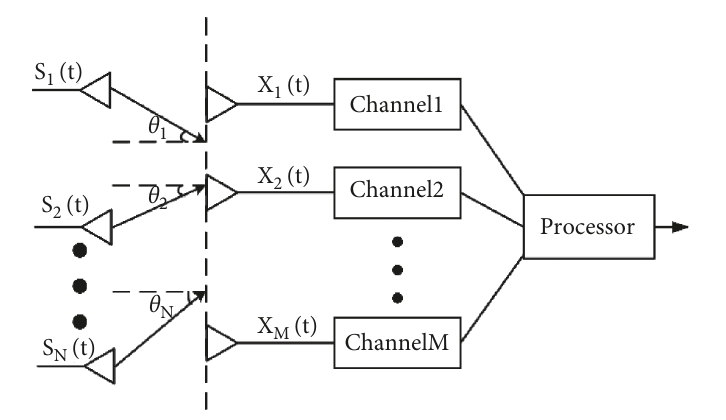
\includegraphics[width=\textwidth]{figures/doa2.png}
    \caption{Diagram of the Electromagnetic Spectrum Monitoring System}
    \label{fig:blocks}
\end{figure}

\begin{figure}[h!]
    \centering
    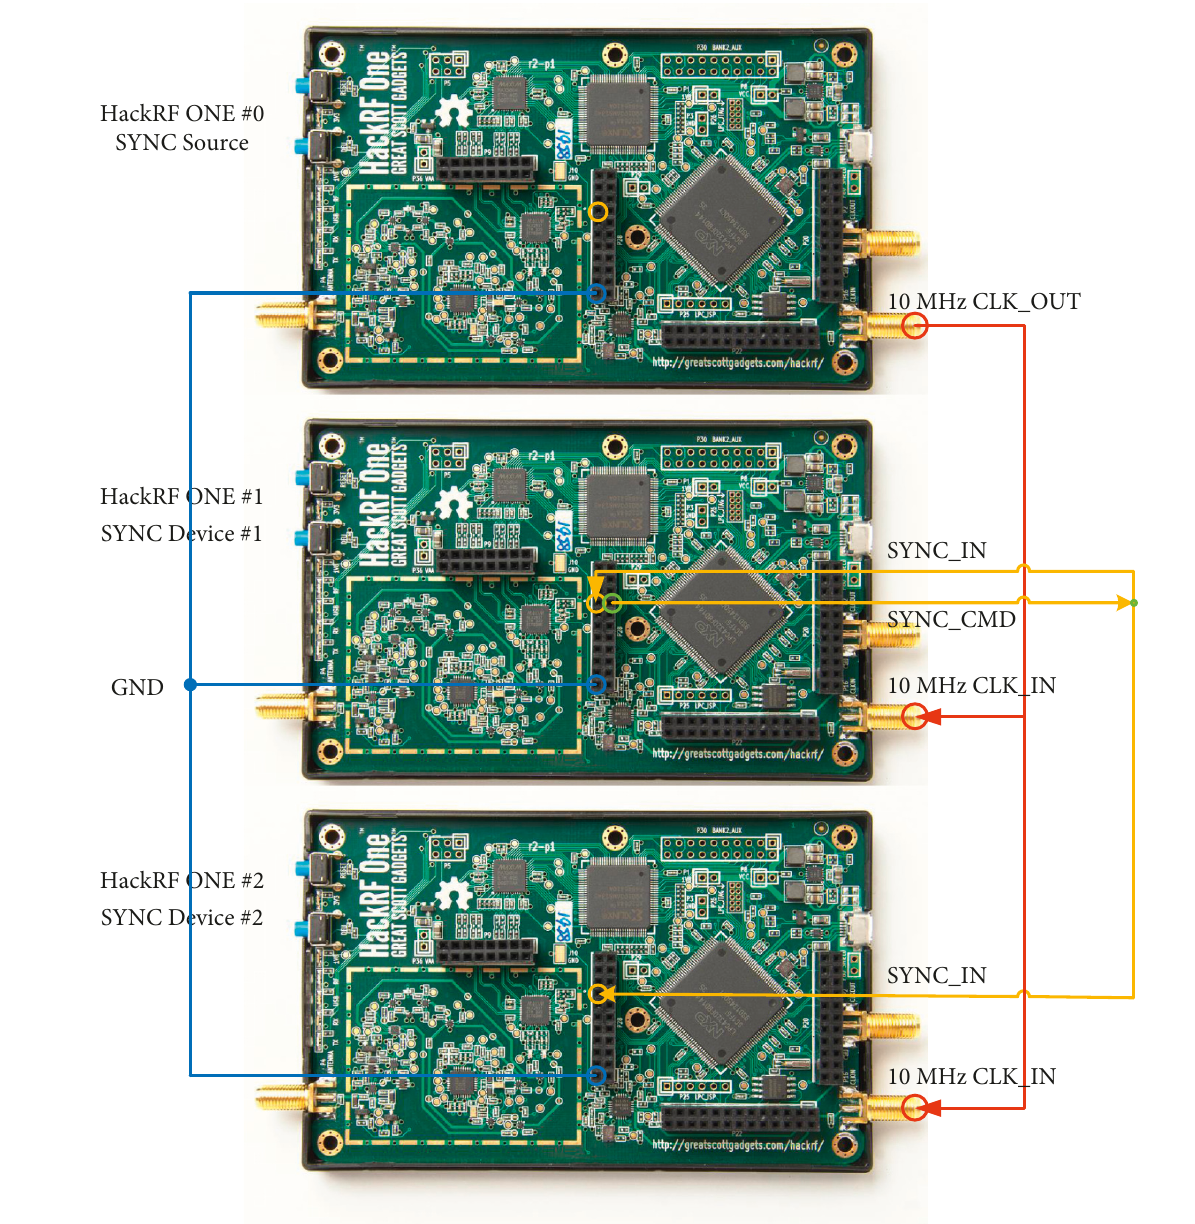
\includegraphics[width=\textwidth]{figures/doa1.png}
    \caption{Diagram of the Electromagnetic Spectrum Monitoring System}
    \label{fig:blocks}
\end{figure}

Additionally, the need for precise synchronization between multiple HackRF One devices introduces complexity into the system setup. Although the authors have implemented effective solutions for clock and time synchronization, this process requires careful calibration and may be susceptible to environmental factors that can introduce synchronization errors.


\begin{figure}[h!]
    \centering
    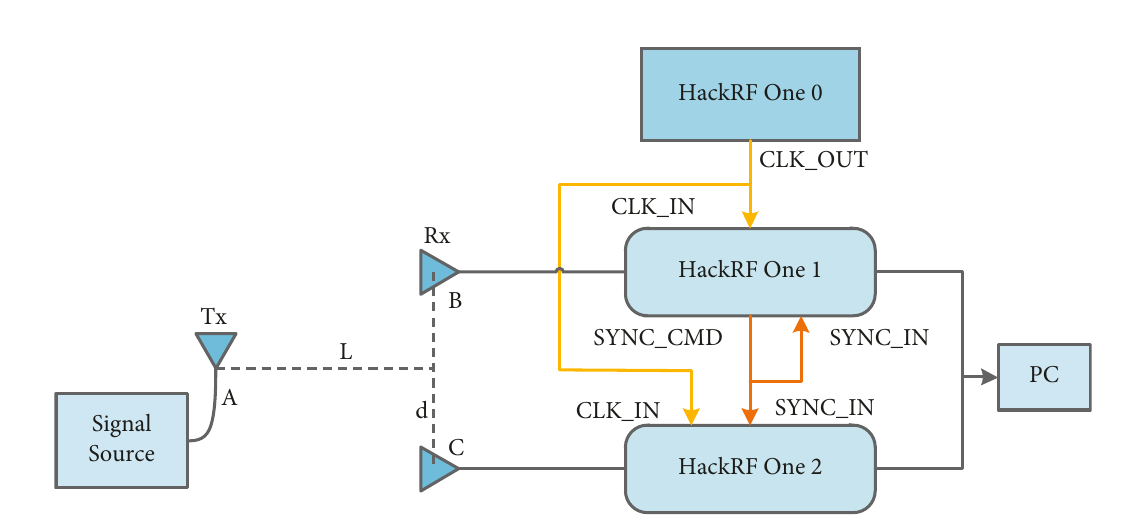
\includegraphics[width=\textwidth]{figures/doa3.png}
    \caption{Diagram of the Electromagnetic Spectrum Monitoring System}
    \label{fig:blocks}
\end{figure}

The dependence on software-defined solutions also means that the system's performance is closely tied to the computational capabilities of the host machine. While the system is designed to be low-cost, achieving high accuracy in real-time applications may require more powerful computing resources, particularly when processing large volumes of data or running complex algorithms like MUSIC.


\begin{figure}[h!]
    \centering
    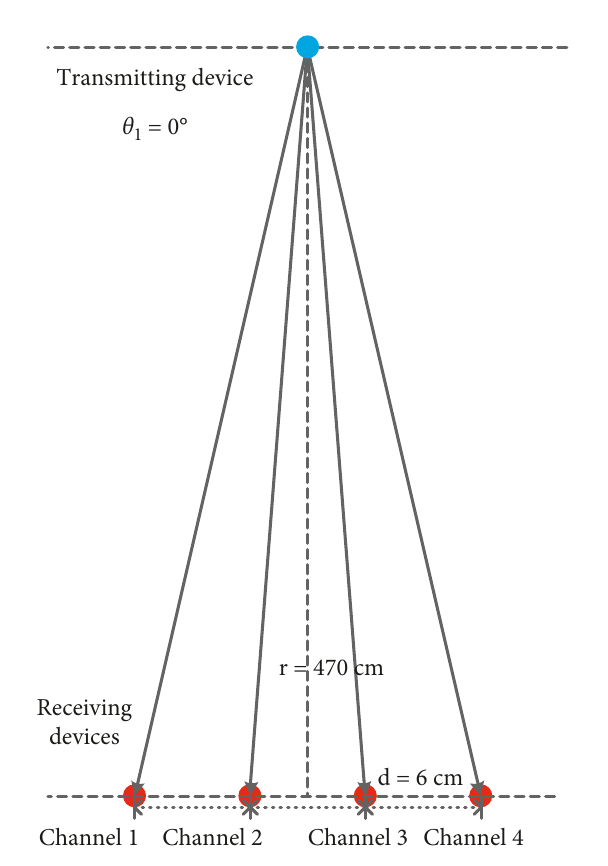
\includegraphics[width=\textwidth]{figures/doa4.png}
    \caption{Diagram of the Electromagnetic Spectrum Monitoring System}
    \label{fig:blocks}
\end{figure}

\subsection{Potential Improvements}

Future work could focus on improving the system's resolution for multiple signal sources by exploring more advanced signal processing algorithms or by enhancing the synchronization mechanism to further reduce phase noise. Additionally, integrating machine learning techniques for adaptive signal processing could help mitigate some of the limitations related to multipath effects and environmental noise.

Another potential improvement is the development of more user-friendly software interfaces that simplify the setup and calibration process, making the system more accessible to non-expert users. This could involve creating automated tools for synchronization calibration or integrating real-time diagnostic tools to monitor system performance during operation.

\subsection{Conclusion}

Overall, the method presented in this paper represents a significant step forward in making DOA estimation technology more accessible and cost-effective. While there are challenges and limitations associated with the use of low-cost SDR devices like HackRF One, the potential applications and benefits of such a system are considerable. With further refinement and development, this approach could become a viable option for a wide range of DOA estimation tasks in various fields, from academic research to practical engineering applications.




\begin{thebibliography}{9}

\bibitem{zhang2022implementation}
Zihan Zhang, Wenjie Zhao, Yonghui Huang, Junshe An, and Yan Zhu, 
``Implementation of DOA Estimation System Based on HackRF One,''
\textit{International Journal of Antennas and Propagation}, 
vol. 2022, no. 1, pp. 7901714, 2022.

\end{thebibliography}








\end{document}


